In the above, we assumed a one-dimensional (1-D) observation, $\bF$.  The raw data, however, is actually a series of multidimensional images. To get the 1-D time-series, two pre-processing steps are required.  First, for each neuron, one must define a region-of-interest (ROI), essentially assigning sets of pixels to neurons. This yields a vector time-series for each neuron, $\vbF_t \in \Real^m$.   Second, one must project the $m-$D observations into a 1-D time-series.  Typically, this step is performed by averaging all the pixels within the ROI.  In theory, one can improve on this uniform averaging by estimating the optimal spatial filter. Here, we provide details on how to incorporate this second step (projecting the $m-$D observations into 1-D) into our fast filter. First, we replace Eq \eqref{eq:obj} with:

\begin{align}
\vbF_t &= \ve{\alpha} C_t + \ve{\beta} +  \ve{\Sig} \ve{\varepsilon}_t, \qquad \varepsilon_t \sim \mathcal{N}(\ve{0},\bI) \label{eq:Obs} 
\end{align}

\noindent where $\vbF_t$, $\ve{\alpha}$, and $\beta$ are all $m$ dimensional column vectors, $\ve{\Sig}$ is the covariance matrix, and $\ve{\varepsilon}_t$ is an $m-$dimensional standard normal random vector. $\Alpha$ now represents the optimal spatial filter, and $\Beta$ represents the baseline for each pixel.  Our goal then is to estimate $\Alpha$ and $\Beta$, to provide maximal information about the underlying spike train.  We would expect this optimal spatial filtering improve the effective SNR after filtering in many situations.  For example, if certain pixels are anti-correlated with others, a uniform spatial filter would average out those differences, whereas the optimal filter would take advantage of that information.    

To estimate $\Alpha$ and $\Beta$, we first plug 
%Then, plugging %To estimate the optimal spatial filter, first we assume that both $\bn$ and $\bC$ are known.  Then, letting $\ve{\eta}_v=[\gam \ve{\Alpha}, \nu \Alpha + \Beta, \rho \Alpha]'$, we see that the parameters are again unidentifiable.  This time, we let $\nu=0$ and $\rho=1$, yielding $\ve{\eta}_v=[\gam \ve{\Alpha}, \Beta,\Alpha]'$.  Then, plugging 
Eqs \eqref{eq:Obs} and \eqref{eq:trans} into \eqref{eq:par1}, to obtain:

\begin{align} 
\vec{\bth} &=\argmax_{\vec{\bth} \in \vec{\bTh}} - \frac{T}{2} \log (2\pi|\ve{\Sig}|) + T\log (\lam \Del) -  \lam \Del \bn' \ve{1} \nonumber\\
&-\frac{1}{2} \sum_{t=1}^T (\vbF_t - \ve{\alpha} (\gamma \hC_{t-1} -\nu  - \rho \hn_t) - \ve{\beta})' \ve{\Sig}^{-1} (\vbF_t - \ve{\alpha} (\gamma \hC_{t-1} -\nu  - \rho \hn_t) - \ve{\beta}) %\nonumber \\
\end{align} 

\noindent where $| \cdot |$ indicates the determinant. By pre-whitening the observation matrix, $\vbF=[\vbF_1, \vbF_2, \ldots, \vbF_T]$, we can estimate the covariance matrix by the identity, i.e., $\ve{\Sig}=\ve{I}$.   Without loss of generality, we may assume that $\nu=0$ and $\rho=1$, similar to our assumption of $\alpha=1$ and $\beta=0$ above. This leaves $\gamma$, $\Alpha$, and $\Beta$. Assuming that $\gamma$ is known (or estimated from the raw fluorescence signal, as we did above), we have: 

\begin{align}
\widehat{\ve{\eta}}_v = \argmax_{\norm{\ve{\eta}_v} <1} \norm{\vbF - \ve{\eta}_v \bX_v}^2 \label{eq:Par}
%\ve{\eta}_v &=\argmax_{\ve{\eta}_v, \, 0 < \gamma < 1} %- \frac{T}{2} \log (2\pi|\ve{\Sig}|) + T \log (\lam \Del) -\lam \Del \bn'\ve{1} 
%-(\vbF -\ve{\eta}_v \bX_v) ' \ve{\Sig}^{-1}   (\vbF - \bX \bth_v) \label{eq:Par}
\end{align}

\noindent where $\ve{\eta}_v=[\Alpha, \, \Beta]$, and $\bX_v=[\gamma \bC + \bn, \, \ve{1}]'$. Note that we have constrained the norm of $\ve{\eta}_v$, which is necessary because otherwise there is a free scale between $\bX_v$ and $\ve{\eta}_v$.  Problems of the form as in Eq \eqref{eq:Par} are known as ``trust region subproblems''.  Fortunately, many algorithms for solving such a problem are available \cite{Fortin00}. 


\begin{figure}[H]
\centering 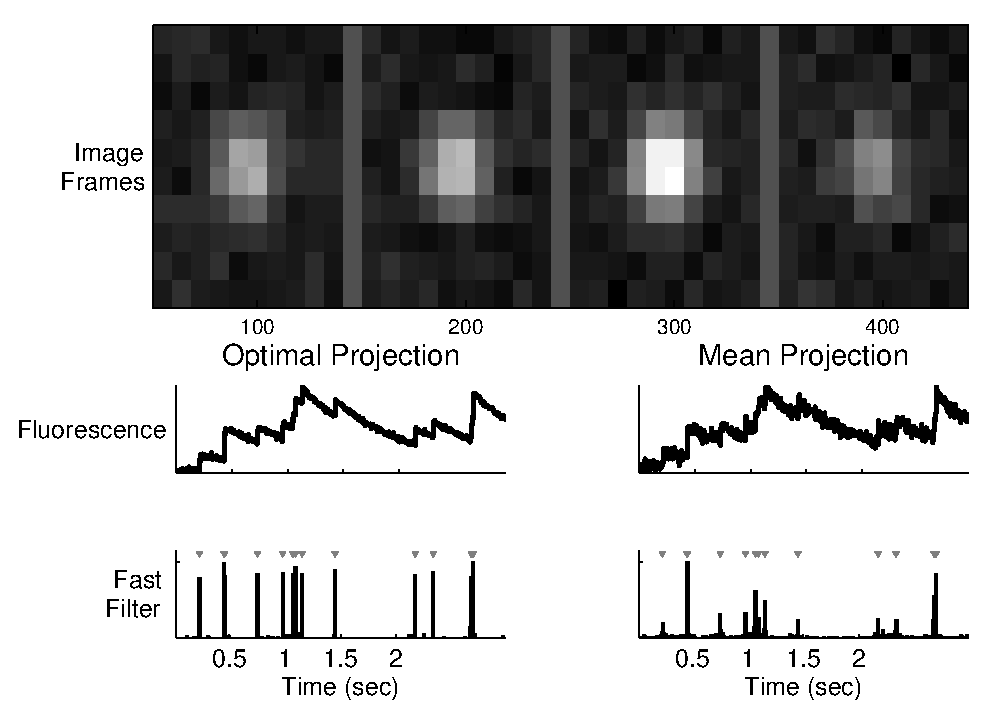
\includegraphics[width=.9\linewidth]{../figs/spatial}
\caption{A simulation demonstrating that using a better spatial filter can significantly enhance the effective SNR (see Supplementary Movie 1 for the full movie associated with this simulation).  Top: five movie frames, equally spaced from the entire move.  Middle left: projection of the entire movie onto the optimal spatial filter, yielding a 1D fluorescence time series, with a small SNR. Bottom left: fast filter's inferred spike train using the optimal spatial filter.  Middle right: projection of the entire movie onto the ``mean'' spatial filter, yielding a 1D fluorescence time series with a large SNR. Bottom right: fast filter's inferred spike train using the mean spatial filter. Parameters different from Fig \ref{fig:schem}: $\balpha$ is a mixture of two Gaussian kernels, each with the same mean, but different variances and component coefficients (see main text for details). $\bbeta=1$.} \label{fig:spatial} \end{figure} 

\begin{figure}[H]
\centering 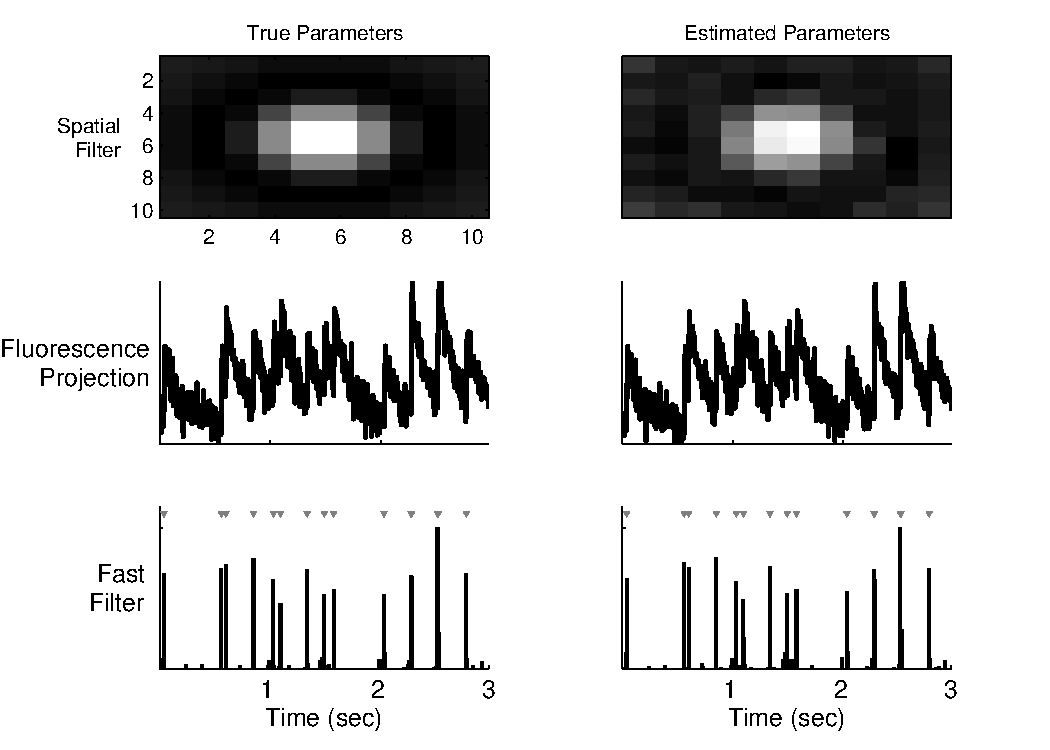
\includegraphics[width=.9\linewidth]{../figs/spatial_EM}
\caption{A simulation demonstrating that given only the fluorescence movie, the parameters may be estimated, and the spike train inferred (c.f. Supplementary Movie 2). Top left panel: true spatial filter.  Middle left panel: projection of movie onto true spatial filter. Bottom left panel: inferred spike train using true parameters. Right panels: same as left except estimating parameters.  $\balpha$ initialized with SVD.  $\bbeta$ initialized with $\ve{0}$.  $\lam$ and $\sig$ were initialized at double their true value.  $\tau$ was assumed known. Parameters same as above.} \label{fig:spatial_EM}
\end{figure}
